\chapter{Objective-C}
\section{Cenni storici}
Nei primi anni ottanta, la pratica comune dell'ingegneria del software era basata sulla programmazione strutturata. Questa modalità era stata sviluppata per poter suddividere programmi di grandi dimensioni in parti più piccole, principalmente per facilitare il lavoro di sviluppo e di manutenzione del software. Ciononostante, col crescere della dimensione dei problemi da risolvere, la programmazione strutturata divenne sempre meno utile, dato che conduceva alla stesura di un numero sempre maggiore di procedure, ad uno spaghetti code e ad uno scarso riuso del codice sorgente.\\\\Venne ipotizzato poi che la programmazione orientata agli oggetti potesse essere una potenziale soluzione al problema. In effetti Smalltalk aveva già affrontato molte di queste questioni ingegneristiche, pur con lo svantaggio di necessitare di una macchina virtuale che interpretava un oggetto in memoria chiamato immagine contenente tutti gli strumenti necessari. L'immagine Smalltalk era molto grossa, usava tendenzialmente un'enorme quantità di memoria per l'epoca e girava molto lentamente anche per la mancanza di un supporto specifico dell'hardware alle macchine virtuali.\\\\Objective C fu creato principalmente da Brad Cox e Tom Love all'inizio degli anni ottanta alla Stepstone. Entrambi erano stati introdotti a Smalltalk durante la loro permanenza al Programming Technology Center della ITT Corporation nel 1981. Cox aveva iniziato ad interessarsi ai problemi legati alla riusabilità del software e si accorse che un linguaggio simile a Smalltalk sarebbe stato estremamente valido per costruire potenti ambiente di sviluppo per i progettisti di ITT.\\\\Cox iniziò così a modificare il compilatore C per aggiungere alcune delle caratteristiche di Smalltalk. Ottenne così ben presto una implementazione funzionante di una estensione ad oggetti del linguaggio C che chiamò OOPC (Object-Oriented Programming in C). Nel frattempo Love fu assunto da Schlumberger Research nel 1982 ed ebbe l'opportunità di acquisire la prima copia commerciale di Smalltalk-80 che influenzò in seguito lo sviluppo della loro creatura.\\\\Per dimostrare che il linguaggio costituiva un reale progresso, Cox mostrò che per realizzare componenti software intercambiabili erano necessari pochi adattamenti pratici agli strumenti già esistenti. Nello specifico, era necessario supportare gli oggetti in modo flessibile con un insieme di librerie software che fossero usabili e consentissero al codice sorgente (e ad ogni risorsa necessaria al codice) di essere raccolto in un solo formato multipiattaforma.\\Cox e Love formarono infine una nuova impresa, la Productivity Products International (PPI), per commercializzare il loro prodotto che accoppiava un compilatore Objective C con una potente classe di librerie.\\\\Nel 1986 Cox pubblicò la sua descrizione dell'Objective C nella sua forma originale nel libro Object-Oriented Programming, An Evolutionary Approach. Sebbene fosse attento a puntualizzare che la questione della riusabilità del software non poteva essere esaurita dal linguaggio di programmazione, l'Objective C si trovò spesso ad essere confrontato, caratteristica per caratteristica, con gli altri linguaggi.\\\\Nel 1988, NeXT, la compagnia fondata da Steve Jobs dopo Apple, ottenne la licenza dell'Objective C da Stepstone (allora proprietaria del marchio) e realizzò il proprio compilatore Objective C e le librerie sulle quali basò l'interfaccia utente di NeXTSTEP. Sebbene le workstation NeXTSTEP non riuscissero ad avere un forte impatto sul mercato, i loro strumenti vennero ampiamente apprezzati dall'industria del settore. Ciò portò NeXT ad abbandonare la produzione di hardware ed a focalizzarsi sugli strumenti software, vendendo NeXTSTEP (e OpenStep) come piattaforma per la programmazione.\\\\In seguito il progetto GNU iniziò a lavorare sul clone libero che chiamò GNUstep, basato sullo standard OpenStep. Dennis Glatting scrisse il primo run-time gnu-objc nel 1992 e Richard Stallman lo seguì subito dopo con un secondo. Il run-time GNU Objective C, che è usato dal 1993, è stato sviluppato da Kresten Krab Thorup mentre era studente universitario in Danimarca.\\
\section{Caratteristiche del linguaggio}
Questo capitolo descrive tutte le funzionalità che il linguaggio aggiunge allo standard C. 
\subsection{Sintassi}
\subsubsection{Implementazione di una classe, i file .h e .m}
L'implementazione di una classe avviene attraverso due file distinti:
\begin{itemize}
\item Un file con estensione .h, che conterrà la dichiarazione dell'interfaccia di classe, i metodi e le properties pubbliche.
\item Un file con estensione .m, che conterrà l'implementazione della classe, la definizione di metodi e properties private; in questo file inoltre saranno definiti i metodi e le variabili d'istanza private.
\end{itemize}
Esempio di file header (.h) di una classe:
\lstset{language=[Objective]C, breakindent=40pt, breaklines}
\begin{lstlisting}
#import <Foundation/Foundation.h>

@interface Persona: NSObject ()

//costruttore personalizzato con parametri 

- (id)initConNome:(NSString *)unNome
      cognome:(NSString *)unCognome;

// dichiarazione delle properties private 

@private
	NSString *_nome;
	NSString *_cognome;
	int _eta; 
}

// dichiarazione dei metodi getter e setter

- (NSString *)nome;
- (void)setNome:(NSString *)nome;
- (NSString *)cognome;
- (void)setCognome:(NSString *)cognome;
- (int)eta;
- (void)setEta:(int)eta;

@end
\end{lstlisting}
\bigskip
\bigskip
\bigskip
Esempio di file di implementazione (.m) di una classe:
\lstset{language=[Objective]C, breakindent=40pt, breaklines}
\begin{lstlisting}
#import "Persona.h" 

@implementation Persona

//implementazione della classe dichiarata in Persona.h

- (id)initConNome:(NSString *)unNome
      cognome:(NSString *)unCognome {
    
    if( self = [super init] )
    {
        _nome = unNome;
        _cognome = unCognome;
    }
    
    return self;
}
 
-(NSString *) nome {
	return _nome
}

-(NSString *) cognome {
	return _cognome
}

-(int) eta {
	return _eta
}

-(void)setNome:(NSString *)nome {
	_nome = nome;
}

-(void)setCognome:(NSString *)cognome {
	_cognome = cognome;
}

-(void)setEta:(int)eta {
	_eta = eta;
}
@end
\end{lstlisting}
\bigskip
\bigskip
\bigskip
Attraverso la parola chiave @property è anche possibile lasciare la definizione dei setter e dei getter al compilatore:
\lstset{language=[Objective]C, breakindent=40pt, breaklines}
\begin{lstlisting}
//come dichiarati in Persona.h
- (NSString *)nome;
- (void)setNome:(NSString *)nome;

//con property diventa
@property NSString * nome;
\end{lstlisting}
\bigskip
\bigskip
\bigskip
Inoltre, attraverso la parola chiave @synthesize, è possibile lasciare al compilatore anche il compito di implementare i setter e i getter di una property che sia stata definita precedentemente:
\lstset{language=[Objective]C, breakindent=40pt, breaklines}
\begin{lstlisting}
//come dichiarati in Persona.m

-(NSString *) nome {
	return _nome
}

-(void)setNome:(NSString *)nome {
	_nome = nome;
}
//con synthesize diventa:

@synthesize nome = _nome; 
\end{lstlisting}
Le properties permettono di accedere ai getter e ai setter utilizzando la notazione puntata, per maggiore leggibilità del codice:
\lstset{language=[Objective]C, breakindent=40pt, breaklines}
\begin{lstlisting}
//senza properties: 

int eta = [persona eta]; 
[persona setEta:22]; 

//con properties: 

int eta = persona.eta;
persona.eta = 22;
\end{lstlisting}
\newpage
\subsubsection{Dichiarazione e definizione dei metodi}
Come visto per la definizione dei setter, una dichiarazione di funzione (metodo) ha la seguente sintassi: 
\lstset{language=[Objective]C, breakindent=40pt, breaklines}
\begin{lstlisting}
//Nell'ordine: (tipoDiRitorno) nomeMetodo:(tipoArg1)nomeArg1;

- (NSInteger)calcolaEta:(NSDate)dataDiNascita;
\end{lstlisting}
Definizione del metodo appena dichiarato: 
\lstset{language=[Objective]C, breakindent=40pt, breaklines}
\begin{lstlisting}
- (NSInteger)calcolaEta:(NSDate)dataDiNascita {

	NSDate* oggi = [NSDate date];
	NSDateComponents* componentiCalendario = [[NSCalendar currentCalendar] 
                                   			components:NSCalendarUnitYear 
                                   			fromDate:dataDiNascita
                                   			toDate:oggi
                                   			options:0];
	
	NSInteger eta = [componentiCalendario year];
	
	return eta;
}
\end{lstlisting}
\subsubsection{Invio dei messaggi}
In Objective-C, a differenza della maggior parte degli altri linguaggi, non si chiama direttamente un metodo, ma si "passa un messaggio" all'oggetto stesso: 
\lstset{language=[Objective]C, breakindent=40pt, breaklines}
\begin{lstlisting}
[persona calcolaEta:dataDiNascita];
\end{lstlisting}
Questo perchè il runtime del linguaggio mantiene traccia di tutti i metodi e delle funzioni che conosce; Ogni componente della lista ha due campi: il nome del metodo (conosciuto come il “selector” dello stesso) e la sua locazione in memoria.\\Quando un oggetto cerca di chiamare un metodo, il comportamento di questo linguaggio è il seguente: compilando il codice, il compilatore ha tradotto il codice della chiamata (ad esempio: 
\lstset{language=[Objective]C, breakindent=40pt, breaklines}
\begin{lstlisting}
[persona calcolaEta:dataDiNascita];
\end{lstlisting}
in \lstset{language=[Objective]C, breakindent=40pt, breaklines}
\begin{lstlisting}
objc_msgSend(persona, @selector(calcolaEta:),dataDiNascita);
\end{lstlisting}
\bigskip
\bigskip
La funzione objc\_msgSend() opera tramite un lookup dinamico: conoscendo il nome del metodo da ricercare scorre la lista per verificare la sua effettiva presenza e, se presente, lo esegue.\\ 
Questo comportamento ha caratteristiche particolari: potremmo far puntare un certo selettore A, che prima puntava al codice per A, ad un codice per un certo B.\\ 
Lo svantaggio è che il tempo di esecuzione è leggermente minore di una chiamata diretta alla parte di codice; si parla comunque di nano secondi di differenza.\\
\\Inoltre il runtime, prima di inviare il messaggio, richiede all’oggetto se il metodo è riconosciuto dallo stesso. Questo significa che l’oggetto può decidere se accettare il messaggio (è anche per questo che si possono inviare messaggi a nil), inoltrarlo ad un oggetto differente, decidere di eseguire codice differente per un metodo specifico.\\Più in dettaglio, quando inviamo un messaggio ad un oggetto, non abbiamo garanzie sul fatto che: \\-Il metodo che andiamo a chiamare non sia necessariamente quello che verrà effettivamente chiamato\\-L’oggetto che riceverà il messaggio non sarà necessariamente quello che vogliamo che risponda.
\subsection{Gestione della memoria}
Objective-C supporta due meccanismi per la gestione della memoria:\\
\\-MMR (Manual retain-release), dove lo sviluppatore gestisce esplicitamente la memoria, tenendo traccia degli oggetti instanziati. E' implementato tramite un modello chiamato Reference Counting, fornito dalla classe NSObject in congiunzione all'ambiente di runtime; è il metodo più obsoleto e più dispendioso in termini di tempo di sviluppo in quanto è un approccio prettamente manuale.\\
\\-ARC (Automatic reference counting), che utilizza lo stesso sistema di tracciamento degli oggetti di MMR, ma aggiunge automaticamente chiamate ai metodi di gestione della memoria a tempo di compilazione. Questo sistema permette di assicurare che gli oggetti abbiano vita il tempo necessario per il loro utilizzo e non oltre, poichè il compilatore genera in automatico anche i metodi di dealloc appropriati.\\E' l'approccio moderno e più utilizzato della gestione della memoria in Objective-C.
\begin{figure}
      \centering
      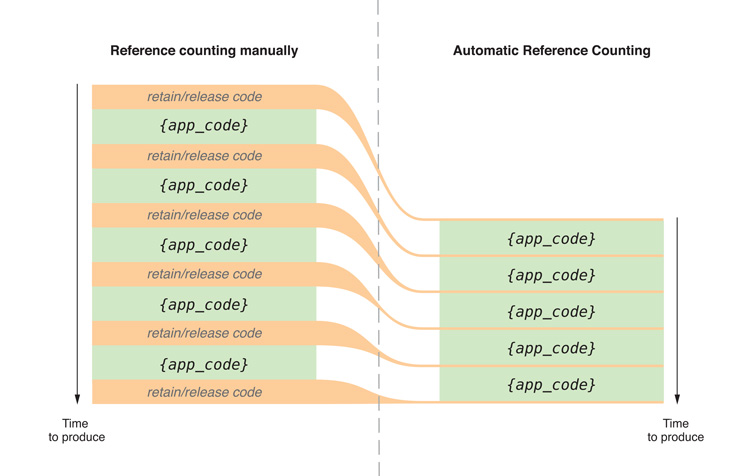
\includegraphics[scale=0.40]{immagini/ARC.jpg}
            \vspace{0.8cm}
            \caption{\textit{Confronto tra MMC ed ARC relativo al tempo di creazione dei cicli di retain-release degli oggetti}}
    \end{figure}
\subsection{Compilatore}
L'IDE di Apple, Xcode, utilizza clang. Quest'ultimo è un compilatore front end per C, C++, Objective-C, Objective-C++, OpenMP, OpenCL e CUDA, basato sul compilatore LLVM (Low Level Virtual Machine).\\
LLVM in origine doveva utilizzare il front end di GCC, ma dopo aver riscontrato problemi di integrazione e di sviluppo l'azienda ha deciso di crearne uno proprio (clang) reso open-source nel Giugno 2007. 
\subsection{Utilizzo in iOS e frameworks Cocoa}
Il linguaggio principale di tutti i frameworks (quali CoreOS, Foundation, CocoaTouch) di iOS e MacOS è ancora Objective-C come dal principio, in quanto Swift non ha ancora raggiunto un livello di maturità tale per essere impiegato per questi scopi (la versione 3 del linguaggio non ha ancora ABI stabili e la sintassi è ancora in corso di modifiche).L'intenzione di Apple è quella di mantenere e migliorare i due linguaggi parallelamente per ancora molto tempo.